\section{Training and Validation Graphs}
\label{sec:training_validation_plots}
The following graphs show the training and validation curves of the models used in this work. They offer a quick view of convergence and stability during fine-tuning without going into detailed discussion.

\subsection{Segment Anything Model (SAM)}
\label{sec:sam_plots}

\autoref{fig:samv1_training_validation} shows the training and validation plots for SAM. The Dice score and IoU improve steadily during training, yet they plateau at modest levels. This indicates that SAM struggles to capture fine morphological details of dendrites, reflecting its limited suitability for the task compared to more advanced variants.

\begin{center}
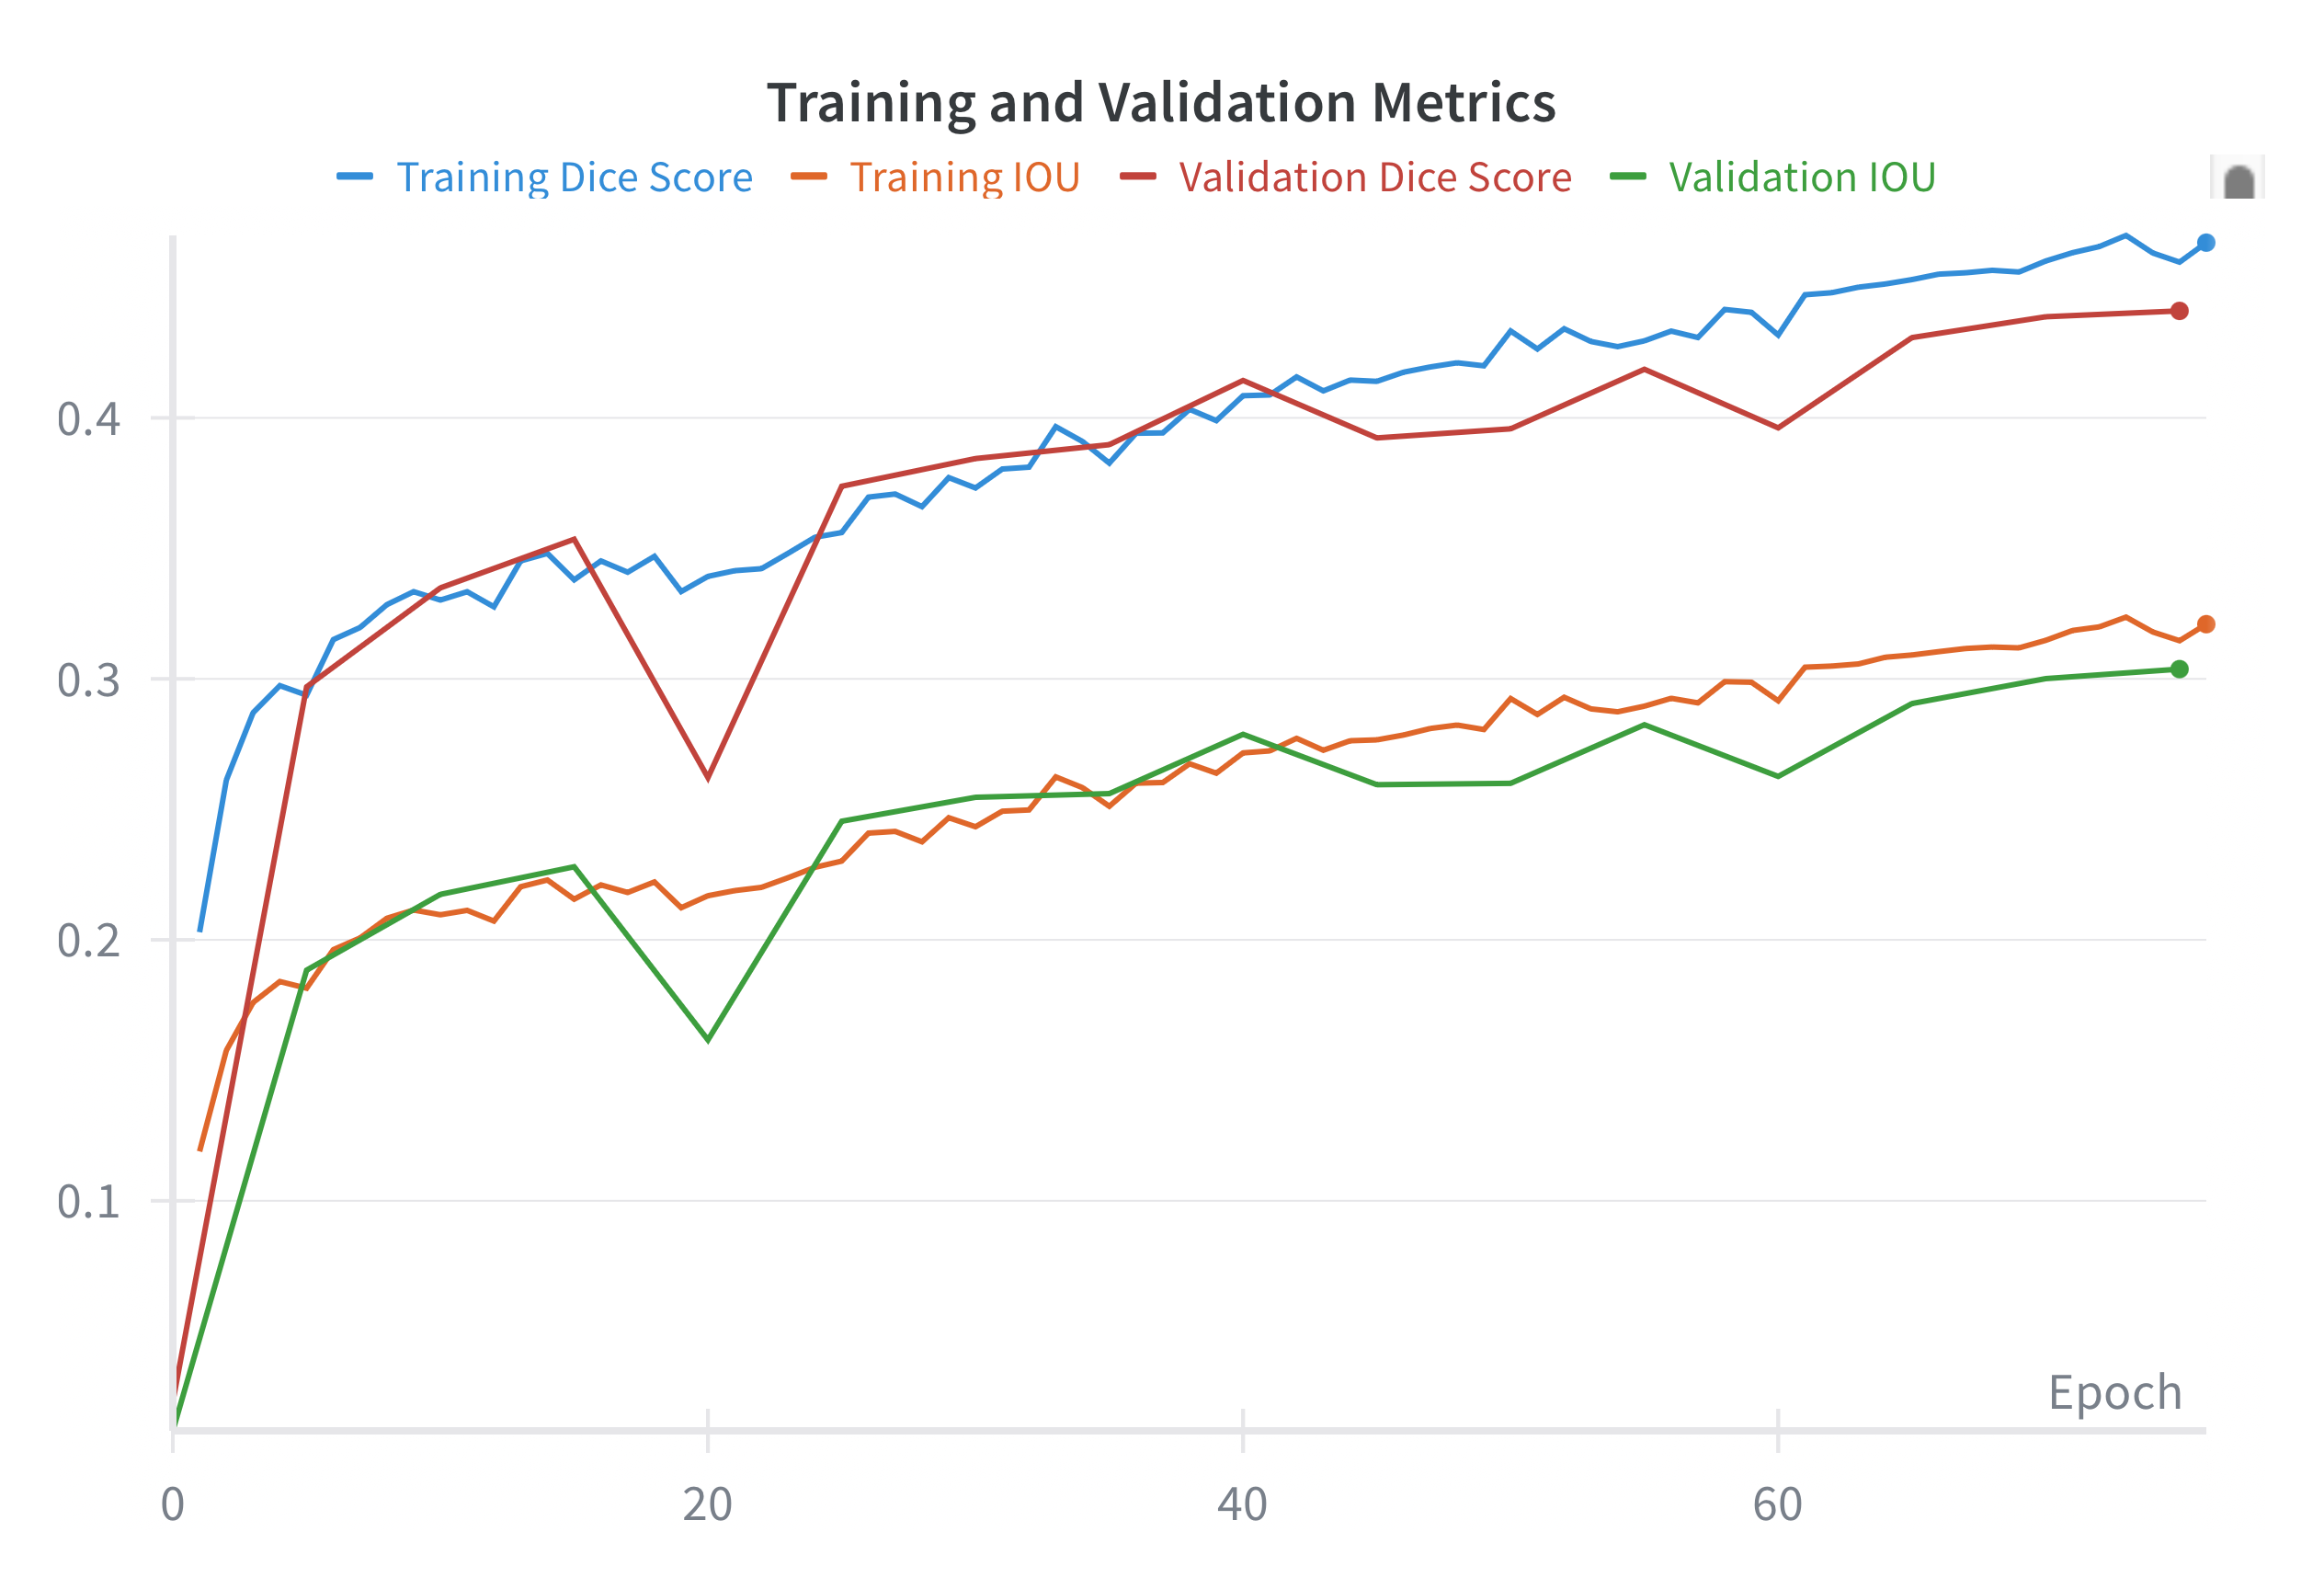
\includegraphics[width=0.8\textwidth]{figures/48_samv1_metrics.png}
\captionof{figure}{Training and Validation Dice and IOU for SAM fine-tuning.}
\label{fig:samv1_training_validation}
\end{center}

In \autoref{fig:samv1_losses}, training and validation losses show a gradual downward trend, but the relatively high values across epochs highlight SAM’s difficulty in effectively minimizing reconstruction error. The gap between training and validation further suggests limited generalization.

\begin{center}
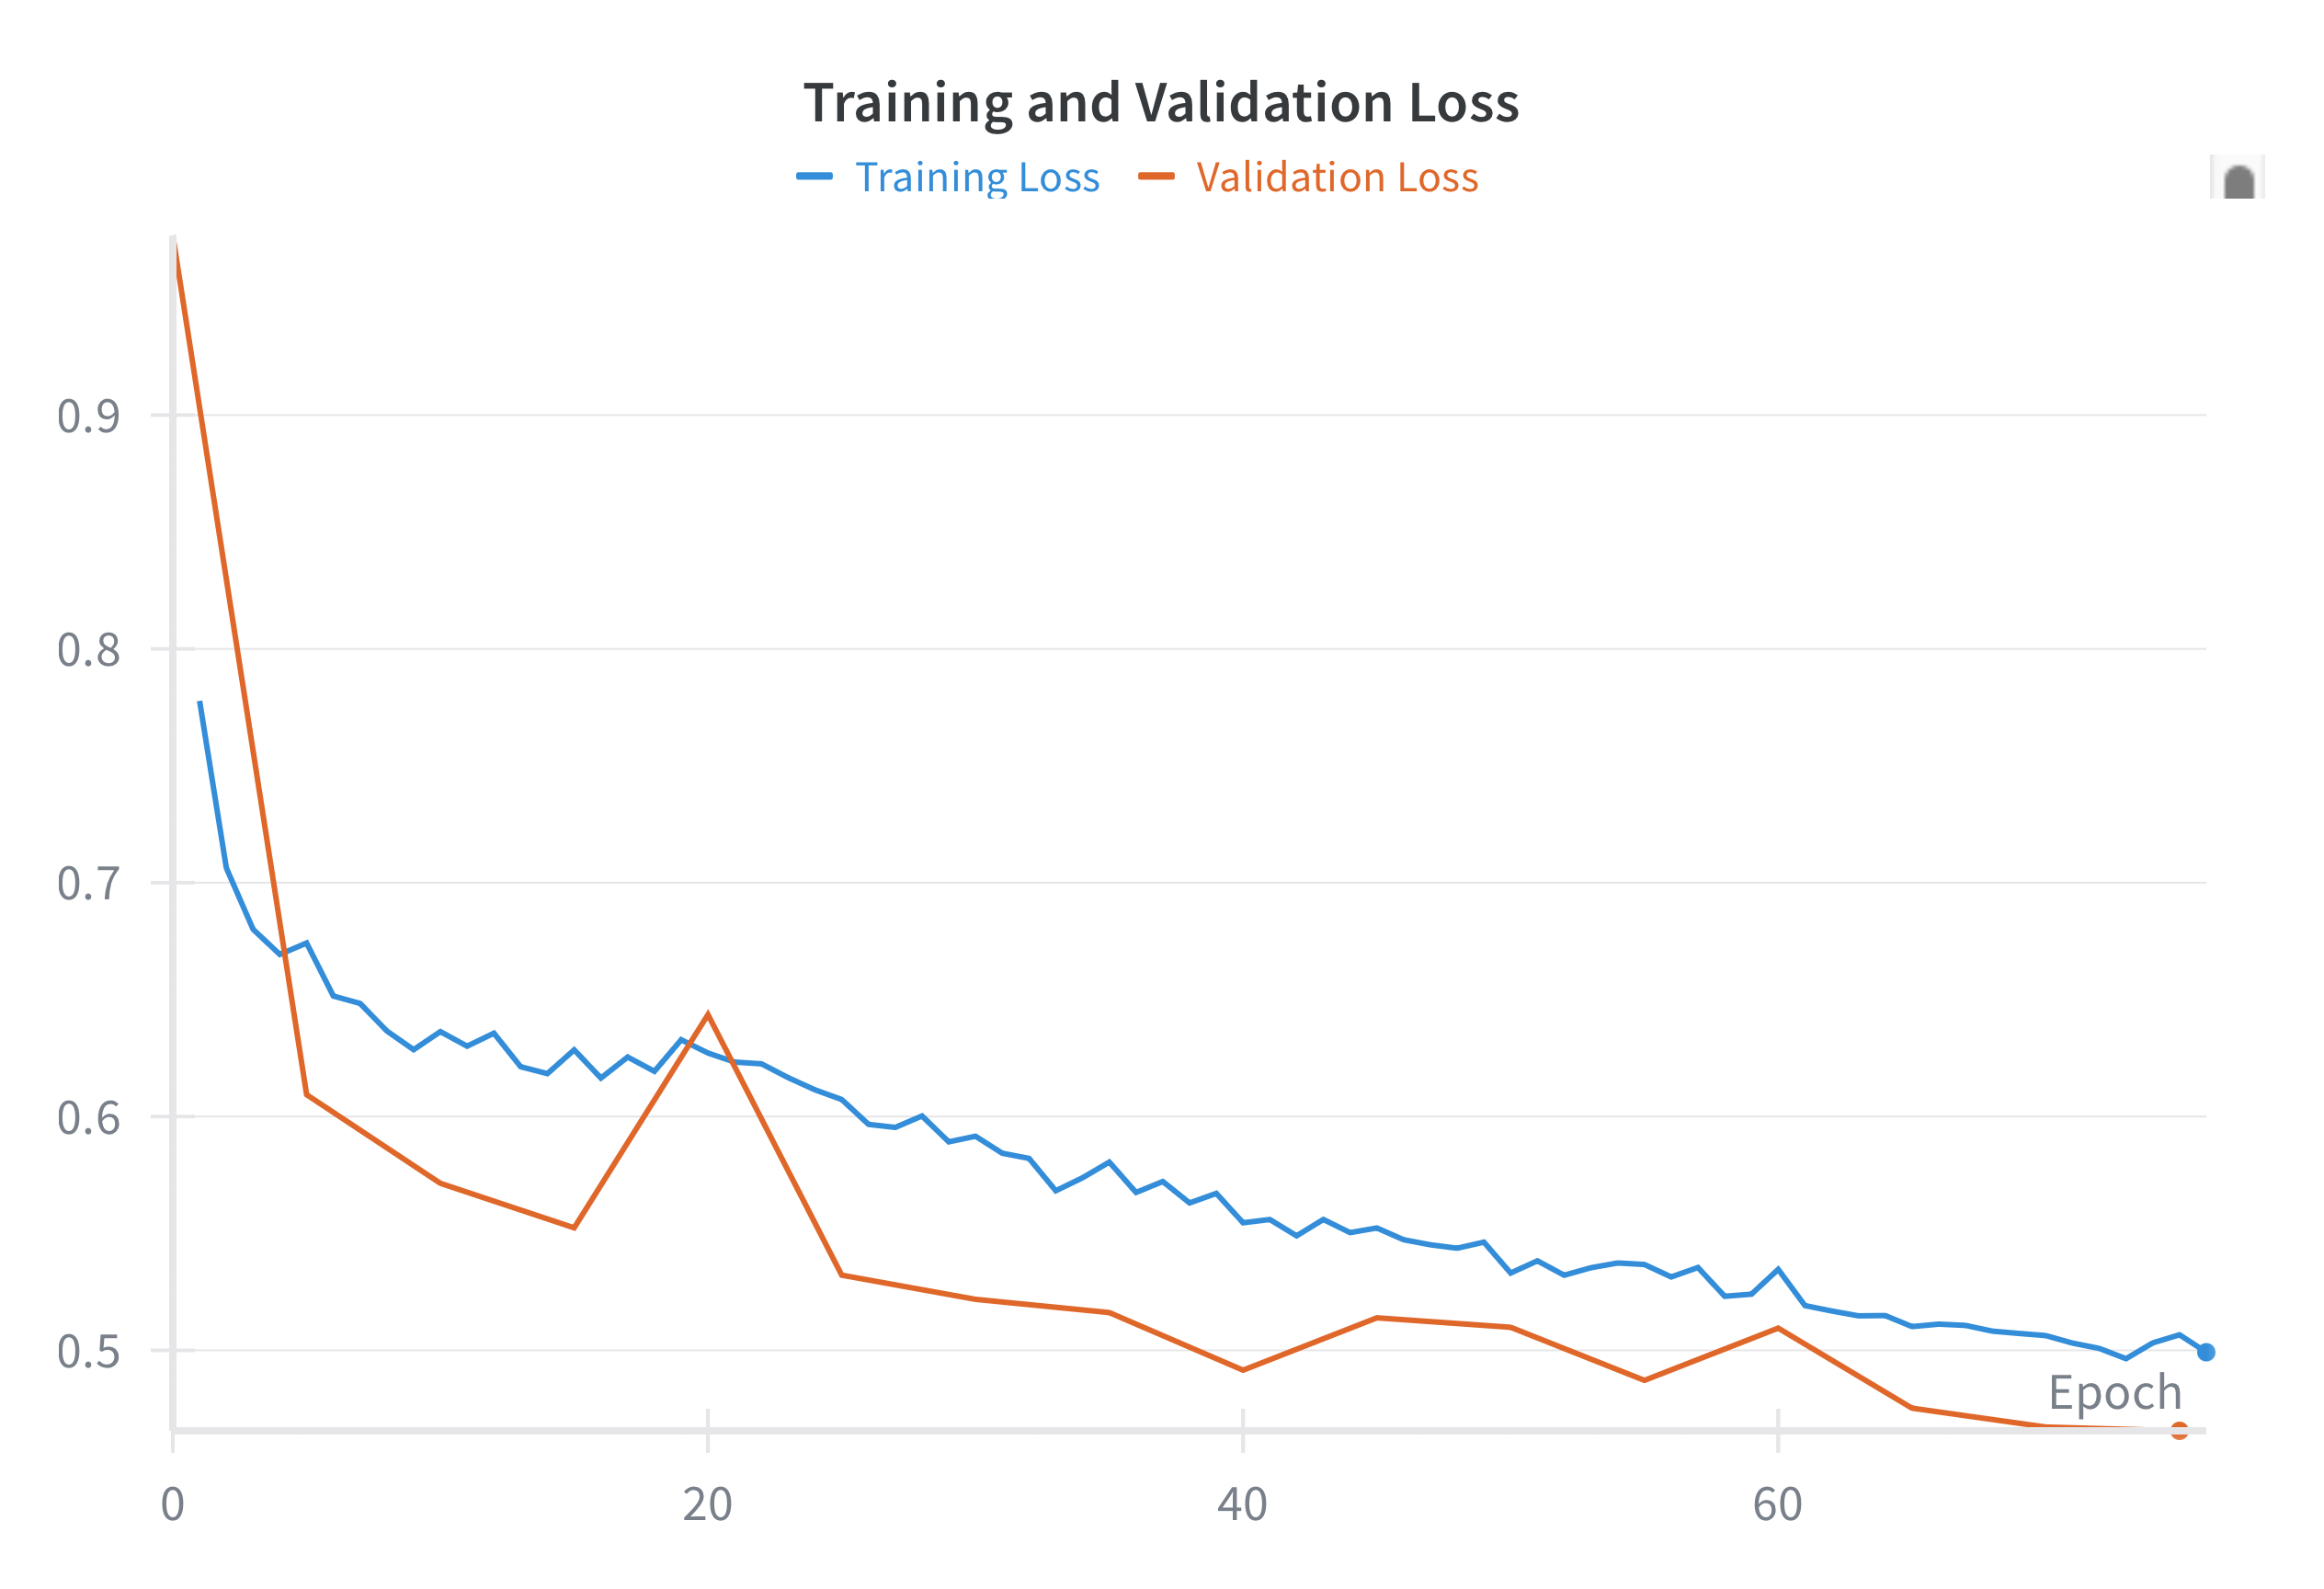
\includegraphics[width=0.8\textwidth]{figures/49_samv1_loss.png}
\captionof{figure}{Training and validation loss curves showing convergence across epochs.}
\label{fig:samv1_losses}
\end{center}


\subsection{SAM + Low Rank Adaptation}
\label{sec:sam_lora_plots}

The Dice and IoU metrics (\autoref{fig:sam_lora_training_validation}) rise quickly in early epochs but stagnate at modest levels. Validation performance consistently lags training, indicating that LoRA adds little benefit over baseline SAM for this task.

\begin{center}
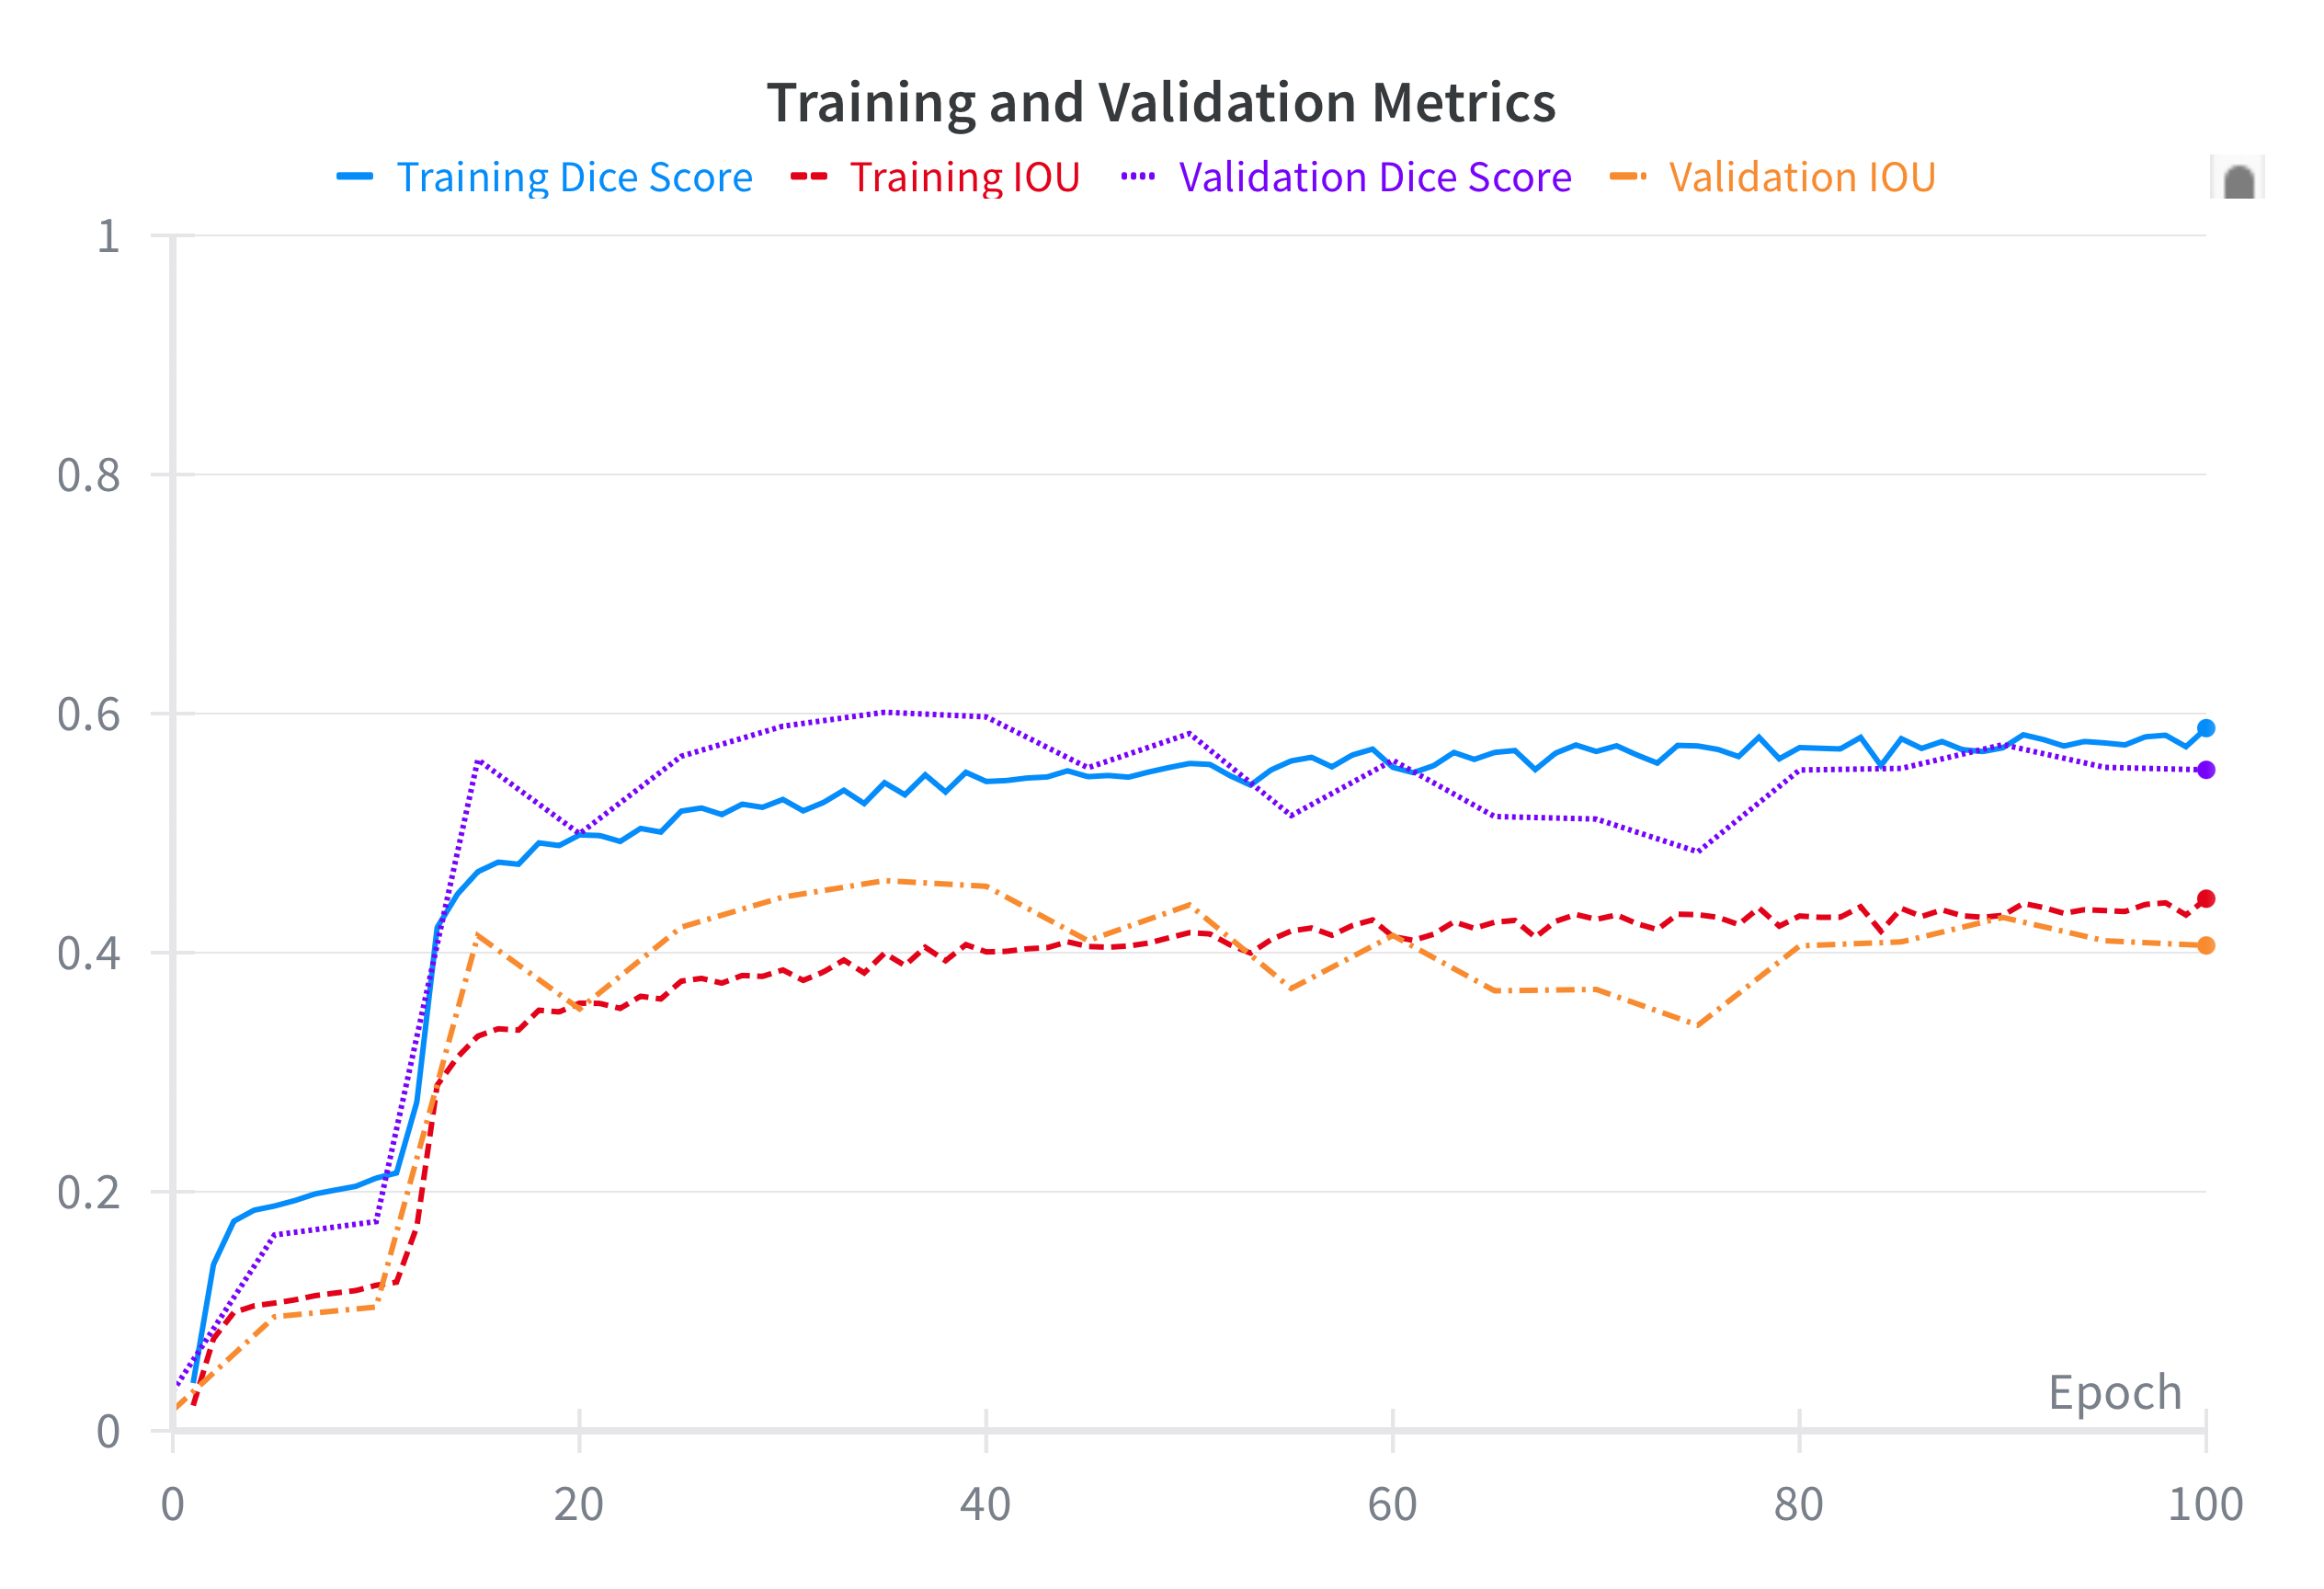
\includegraphics[width=0.8\textwidth]{figures/51_sam_lora_metrics.png}
\captionof{figure}{Training and Validation Dice and IOU for SAM fine-tuning.}
\label{fig:sam_lora_training_validation}
\end{center}


SAM+LoRA shows an initial drop in loss, but convergence is unstable at relatively high values (\autoref{fig:sam_lora_losses}). The noisy validation curve suggests weak generalization and poor stability during training.
\begin{center}
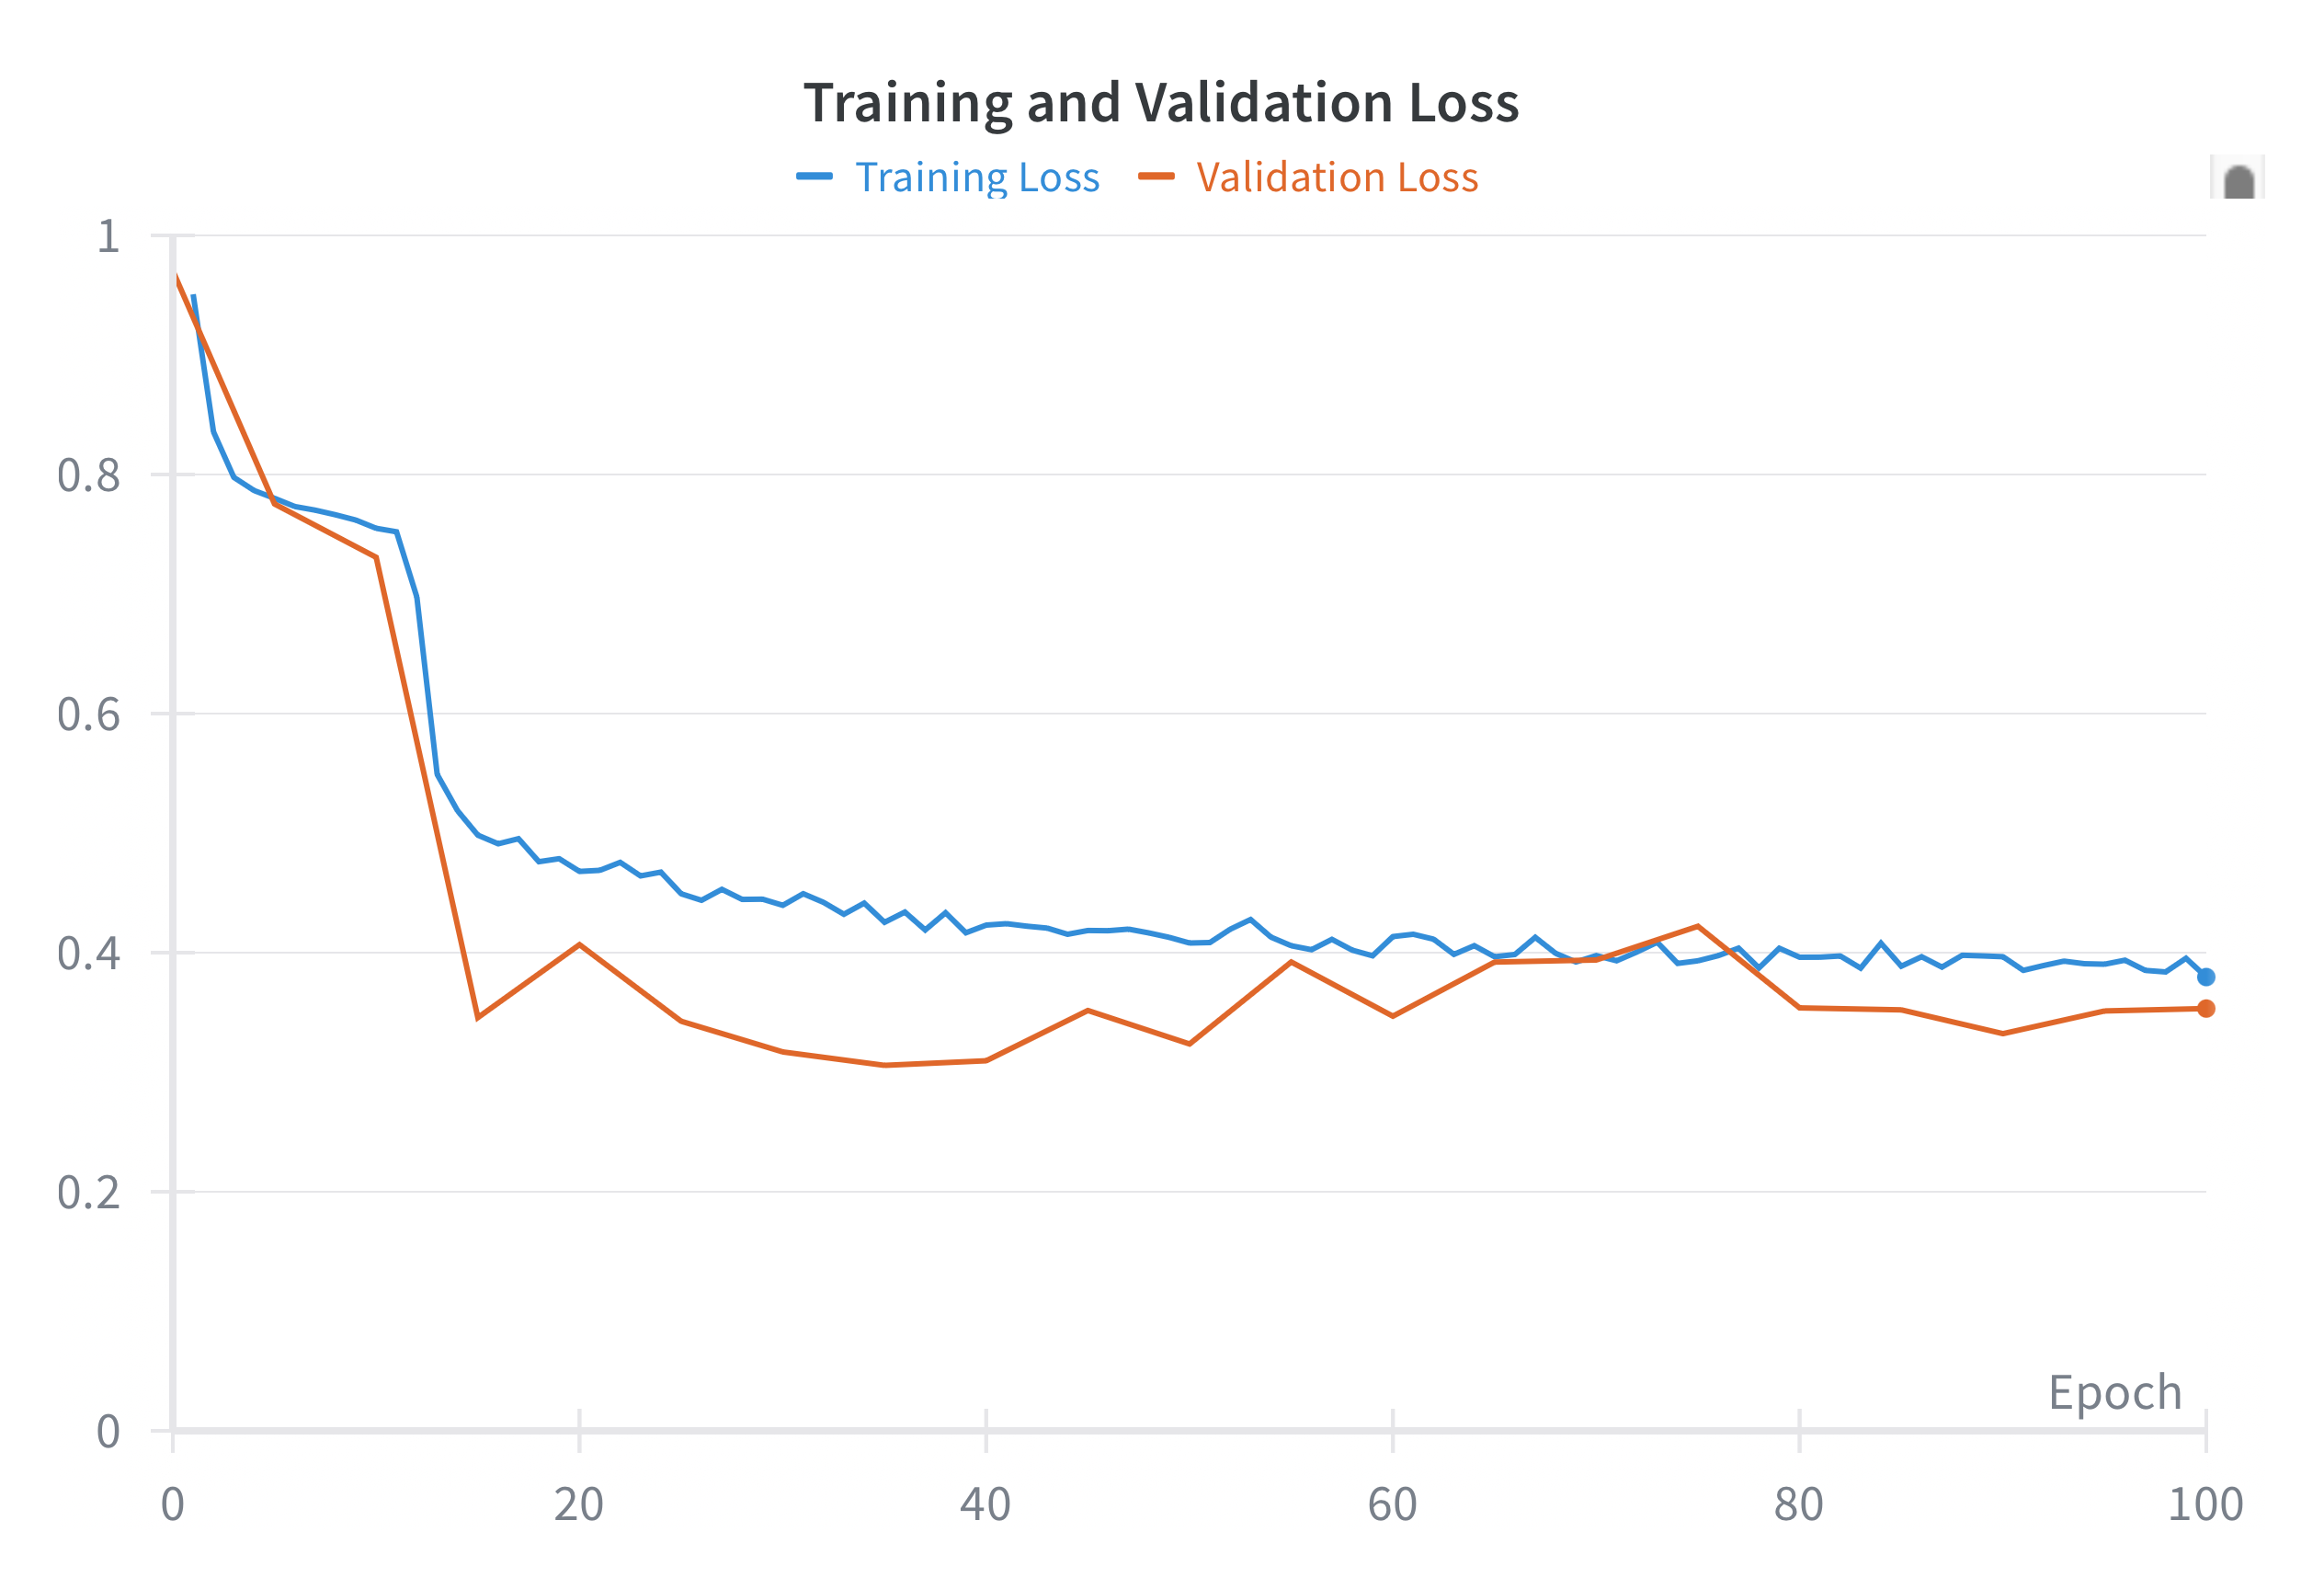
\includegraphics[width=0.8\textwidth]{figures/50_sam_lora_loss.png}
\captionof{figure}{Training and Validation Dice and IOU for SAM fine-tuning.}
\label{fig:sam_lora_losses}
\end{center}


\subsection{Segment Anything Model 2}
\label{sec:sam2_plots}

The following are the training and validation metrics for the Segment Anything Model 2, a key part of the \textbf{Neuro-SAM} pipeline. Since we trained the model on two different datasets, dendrites and dendritic spine; we will analyze their fine-tuning metrics separately. 

\paragraph{SAMv2 Dendrite Fine-Tuning}

The Dice score and IoU rapidly increase and stabilize at substantially higher values than earlier variants. Validation closely tracks training, showing reduced overfitting and improved robustness. These results highlight SAMv2’s superior capacity for capturing dendrite morphology.


\begin{center}
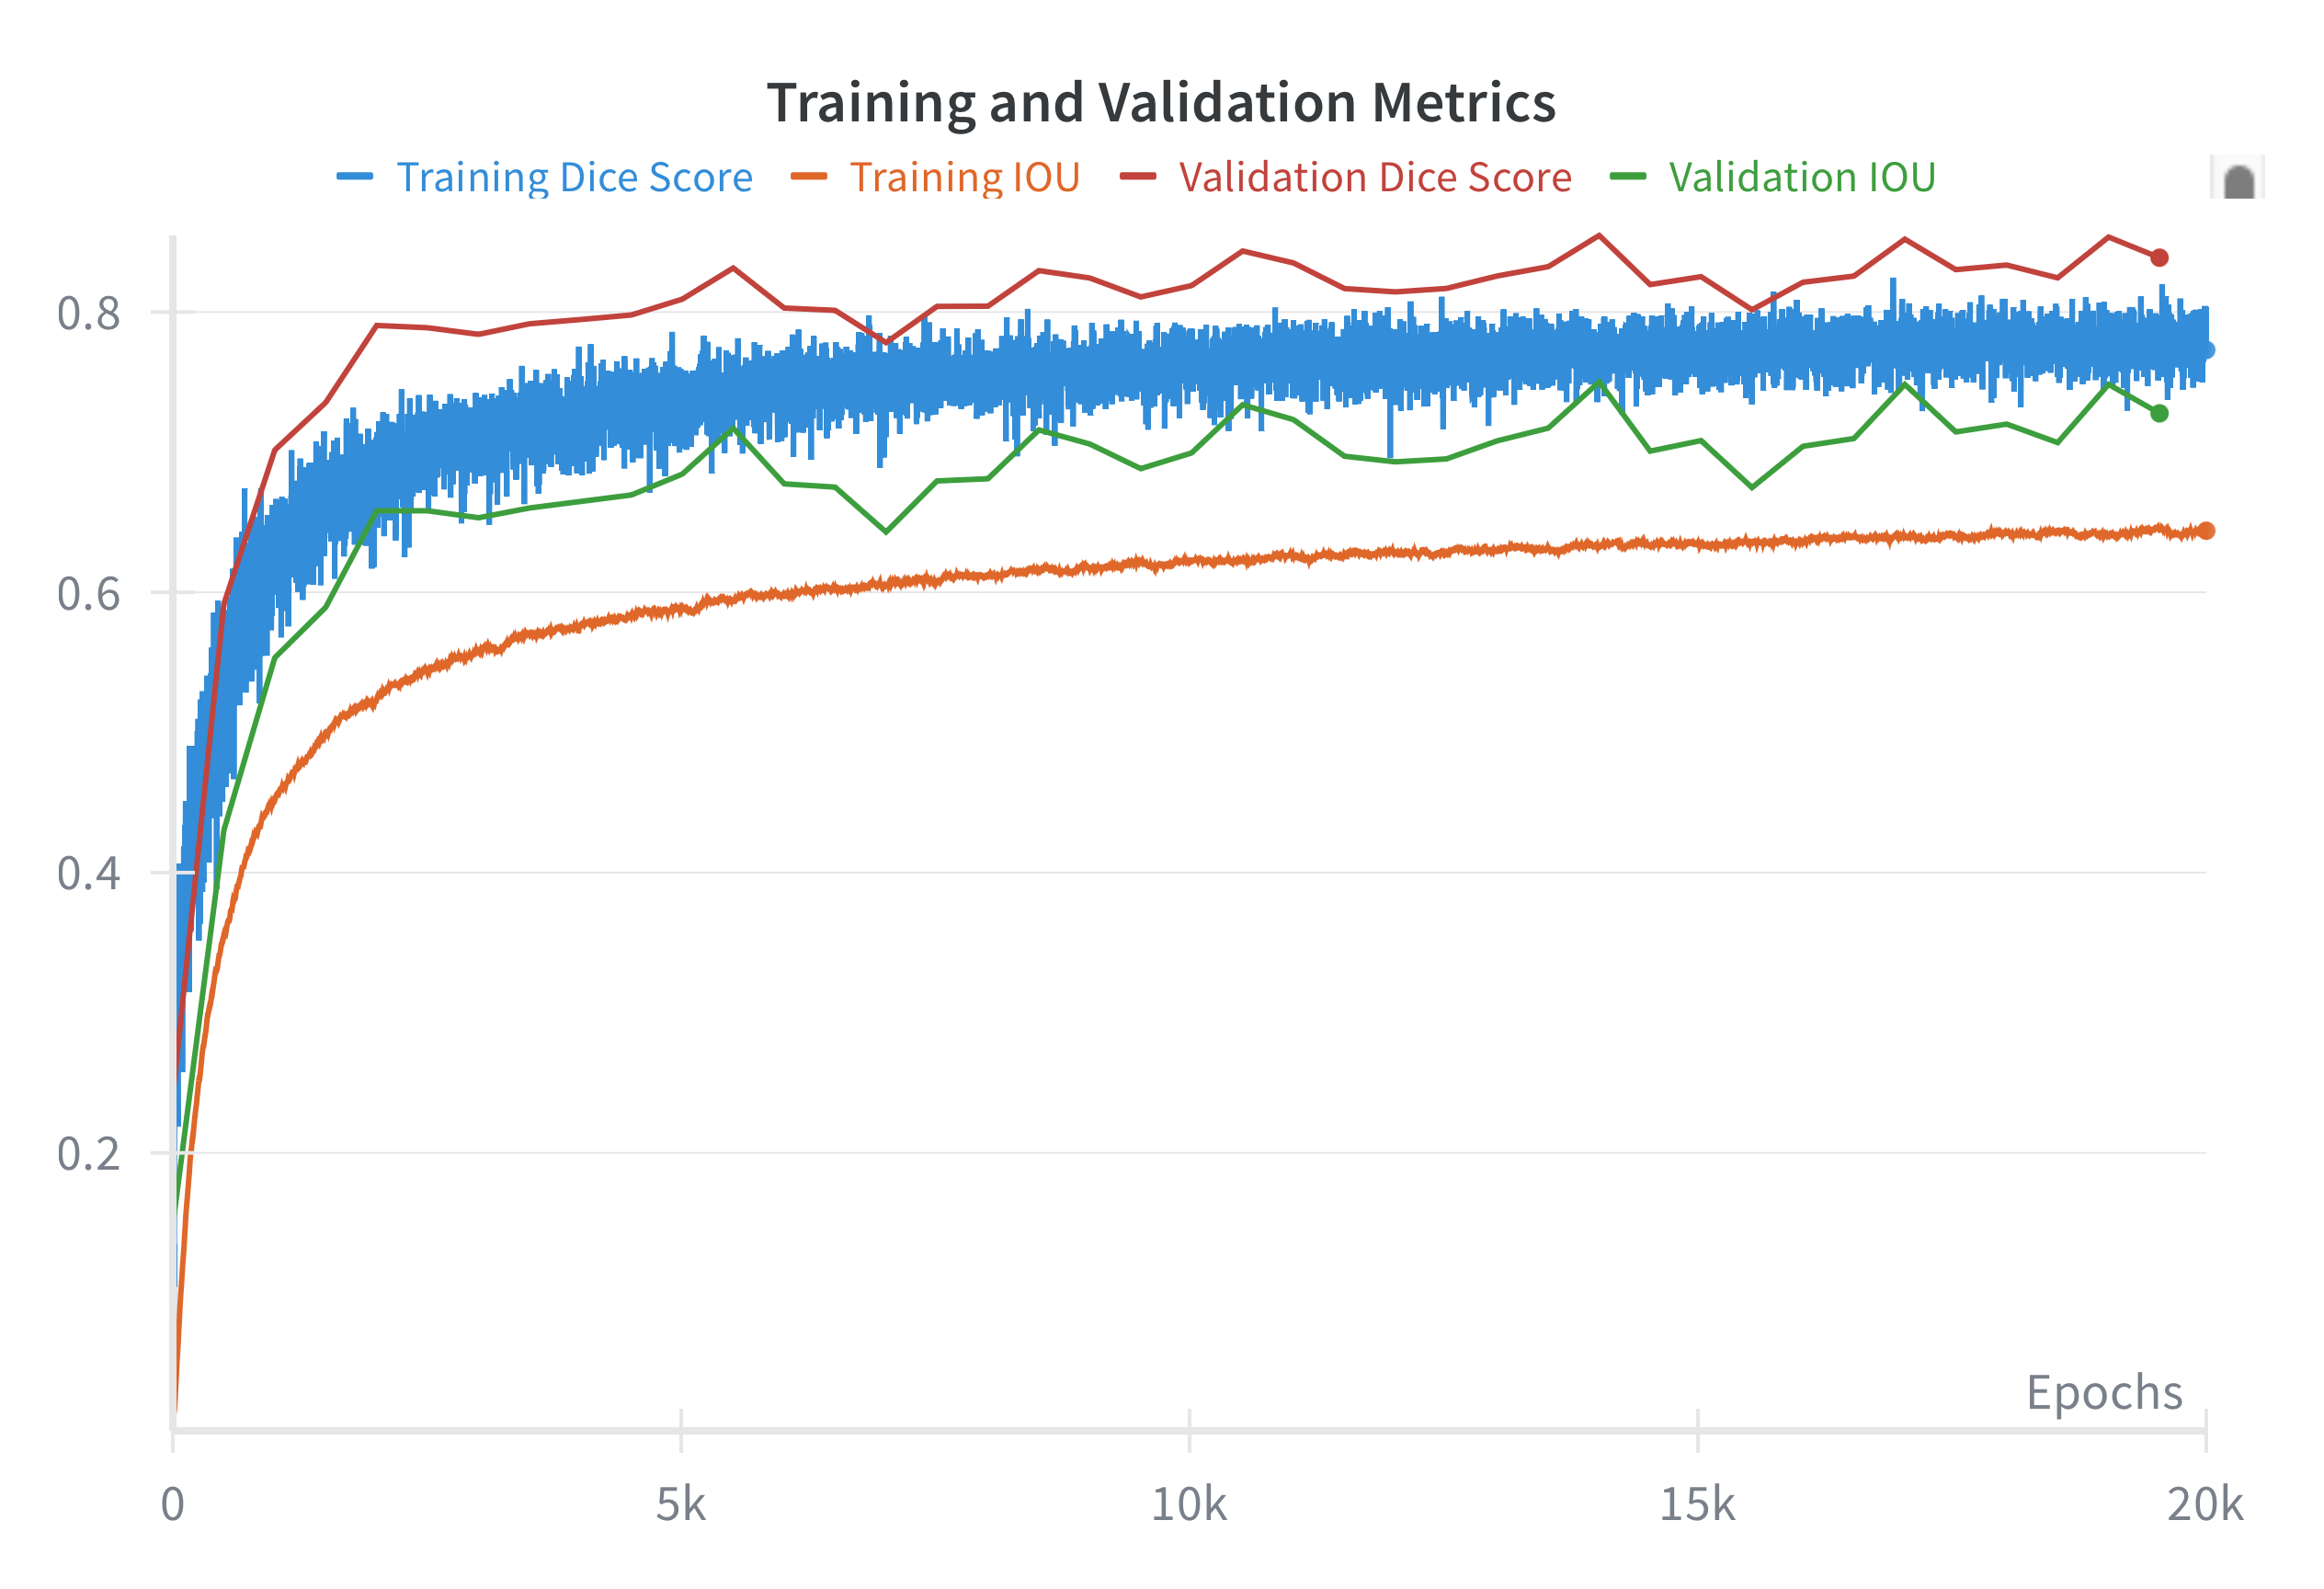
\includegraphics[width=0.8\textwidth]{figures/52_samv2_dendrites_metrics.png}
\captionof{figure}{Training and validation Dice score and IoU for SAMv2, indicating strong improvements and stable performance.}
\label{fig:samv2_dendrite_training_validation}
\end{center}

The SAMv2 loss curves demonstrate clear and stable convergence, with both training and validation losses consistently decreasing to low values. Unlike SAM and SAM+LoRA, the fluctuations remain minimal, reflecting better optimization and stronger generalization.

\begin{center}
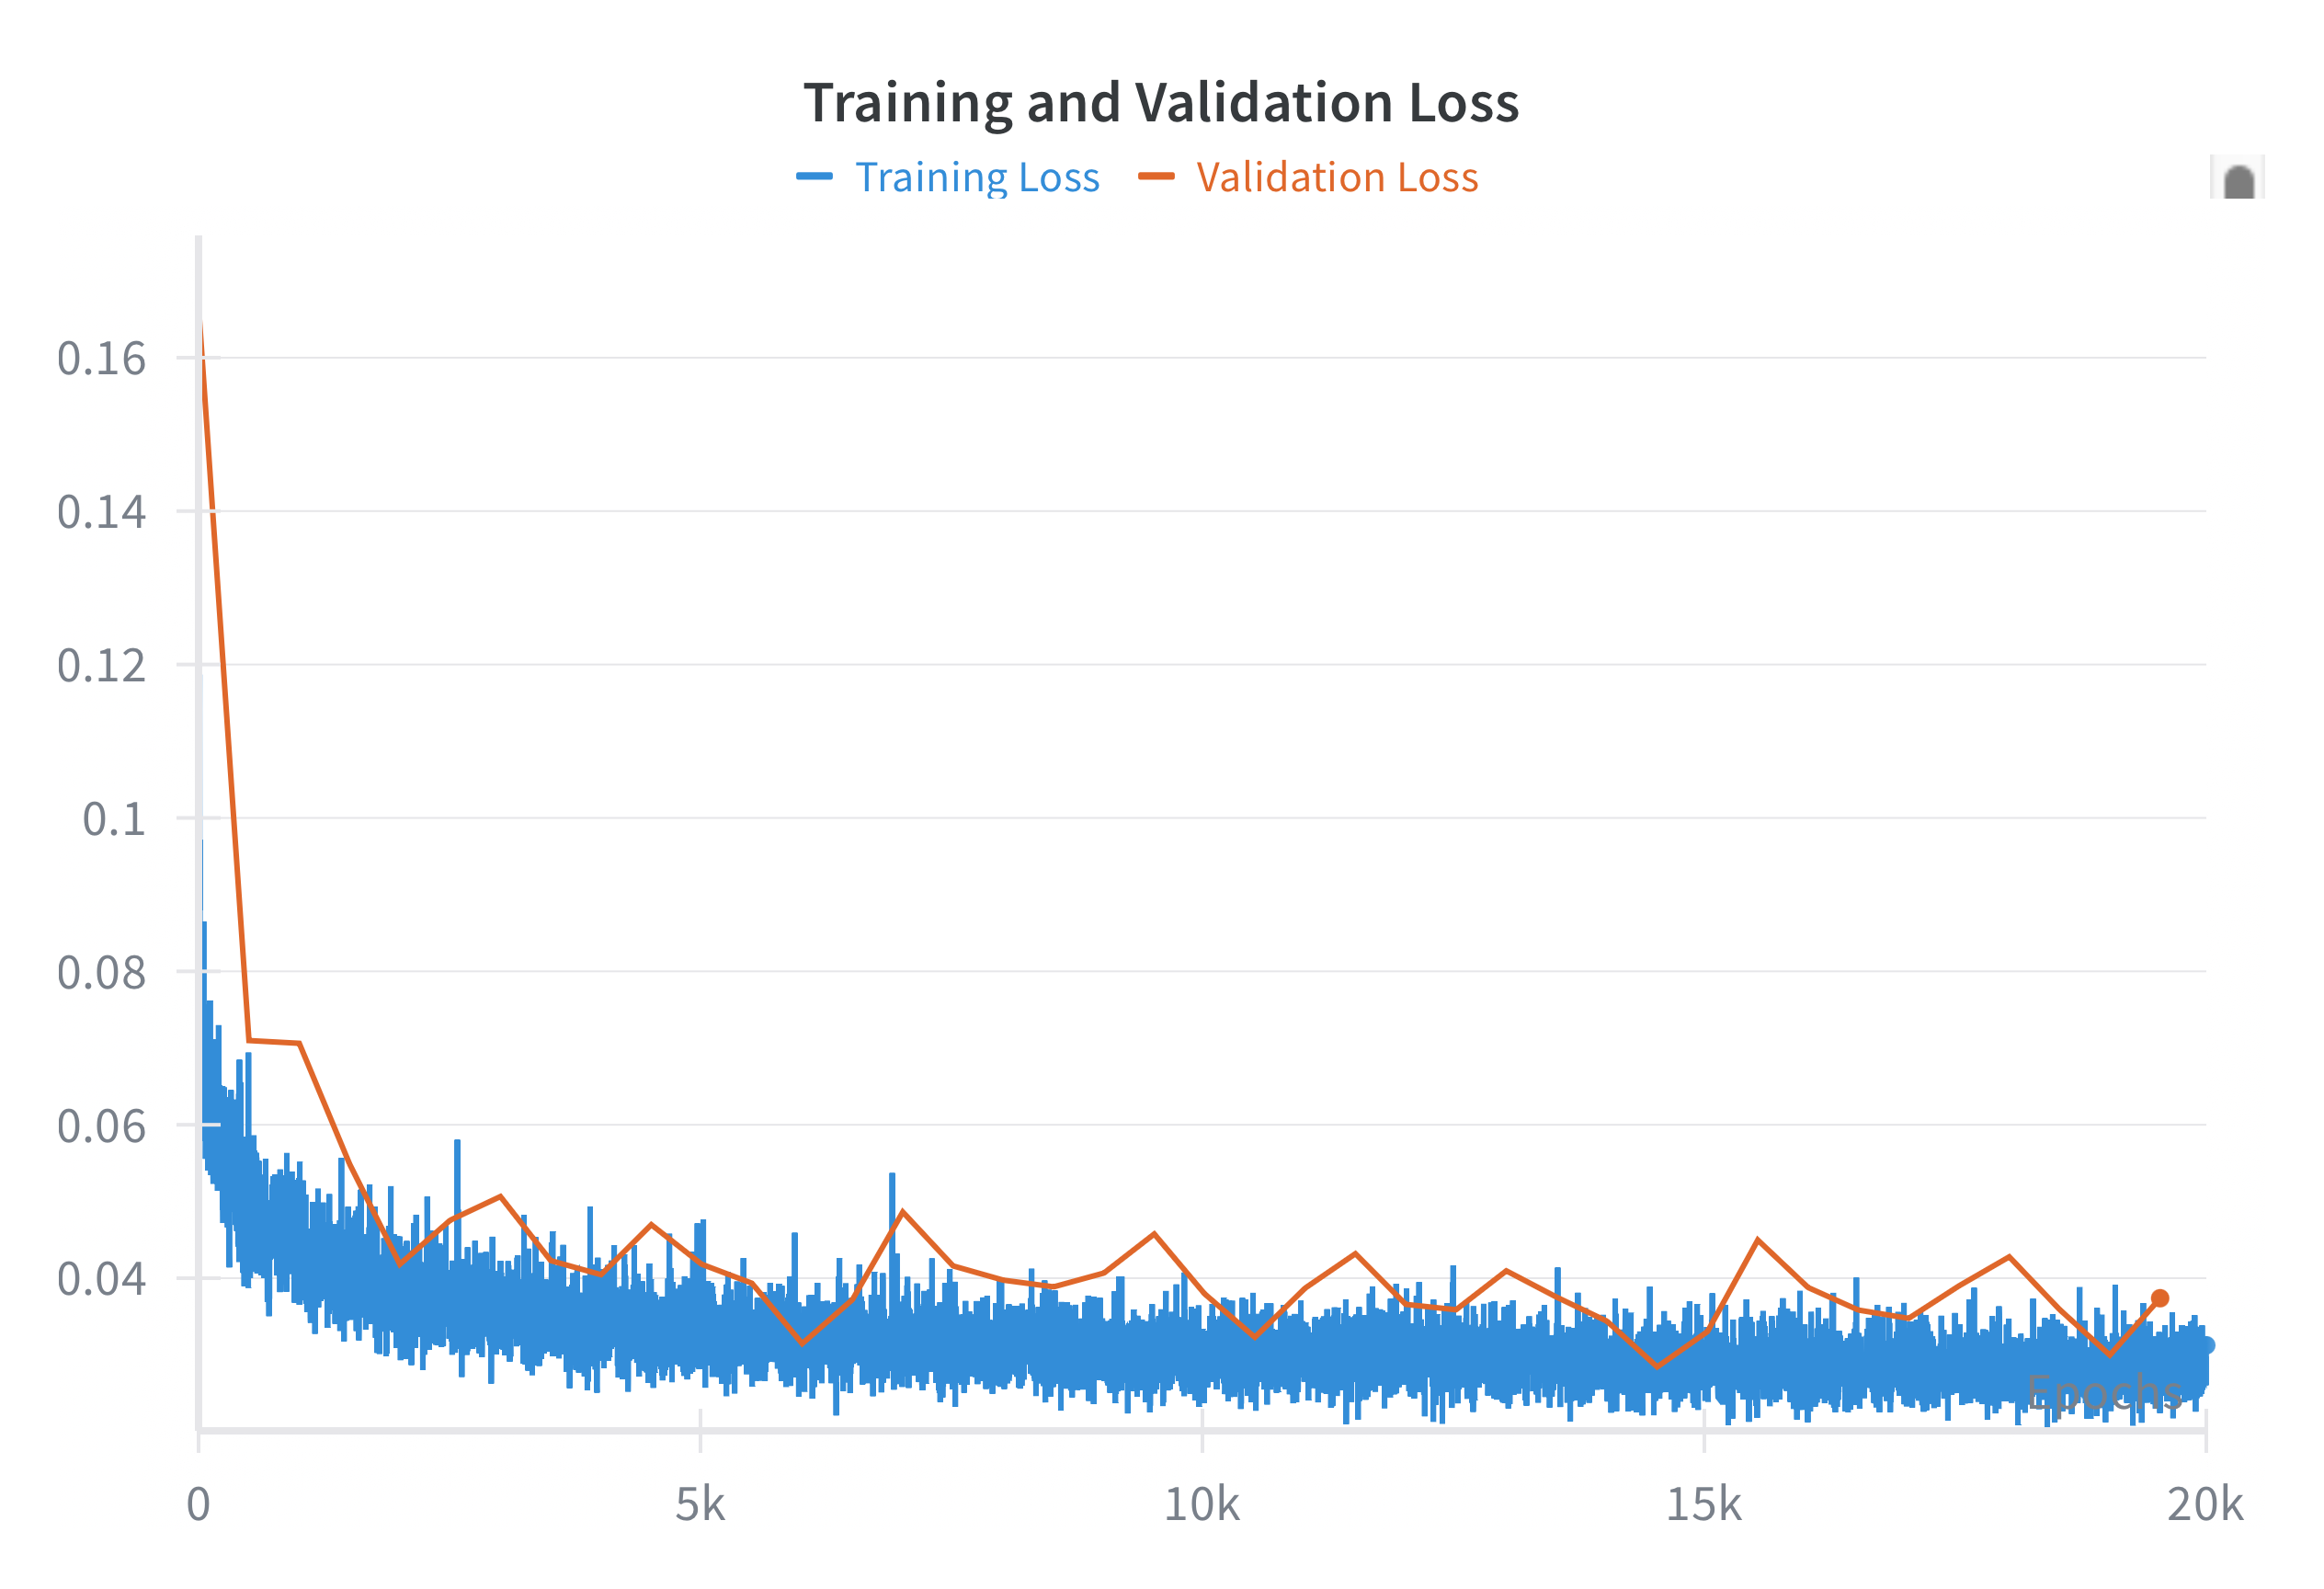
\includegraphics[width=0.8\textwidth]{figures/53_samv2_dendrites_loss.png}
\captionof{figure}{Training and validation loss for SAMv2 fine-tuning on dendrites, showing smooth convergence with low final error.}
\label{fig:samv2_dendrite_loss}
\end{center}


\paragraph{SAMv2 Dendritic Spine Fine-Tuning}
\newline
Metrics improve quickly in early epochs, yet the Dice score and IoU plateau at modest values. Validation lags behind training, indicating persistent overfitting and weaker generalization. These results highlight the greater difficulty of spine segmentation compared to dendrites, even for SAMv2.

\begin{center}
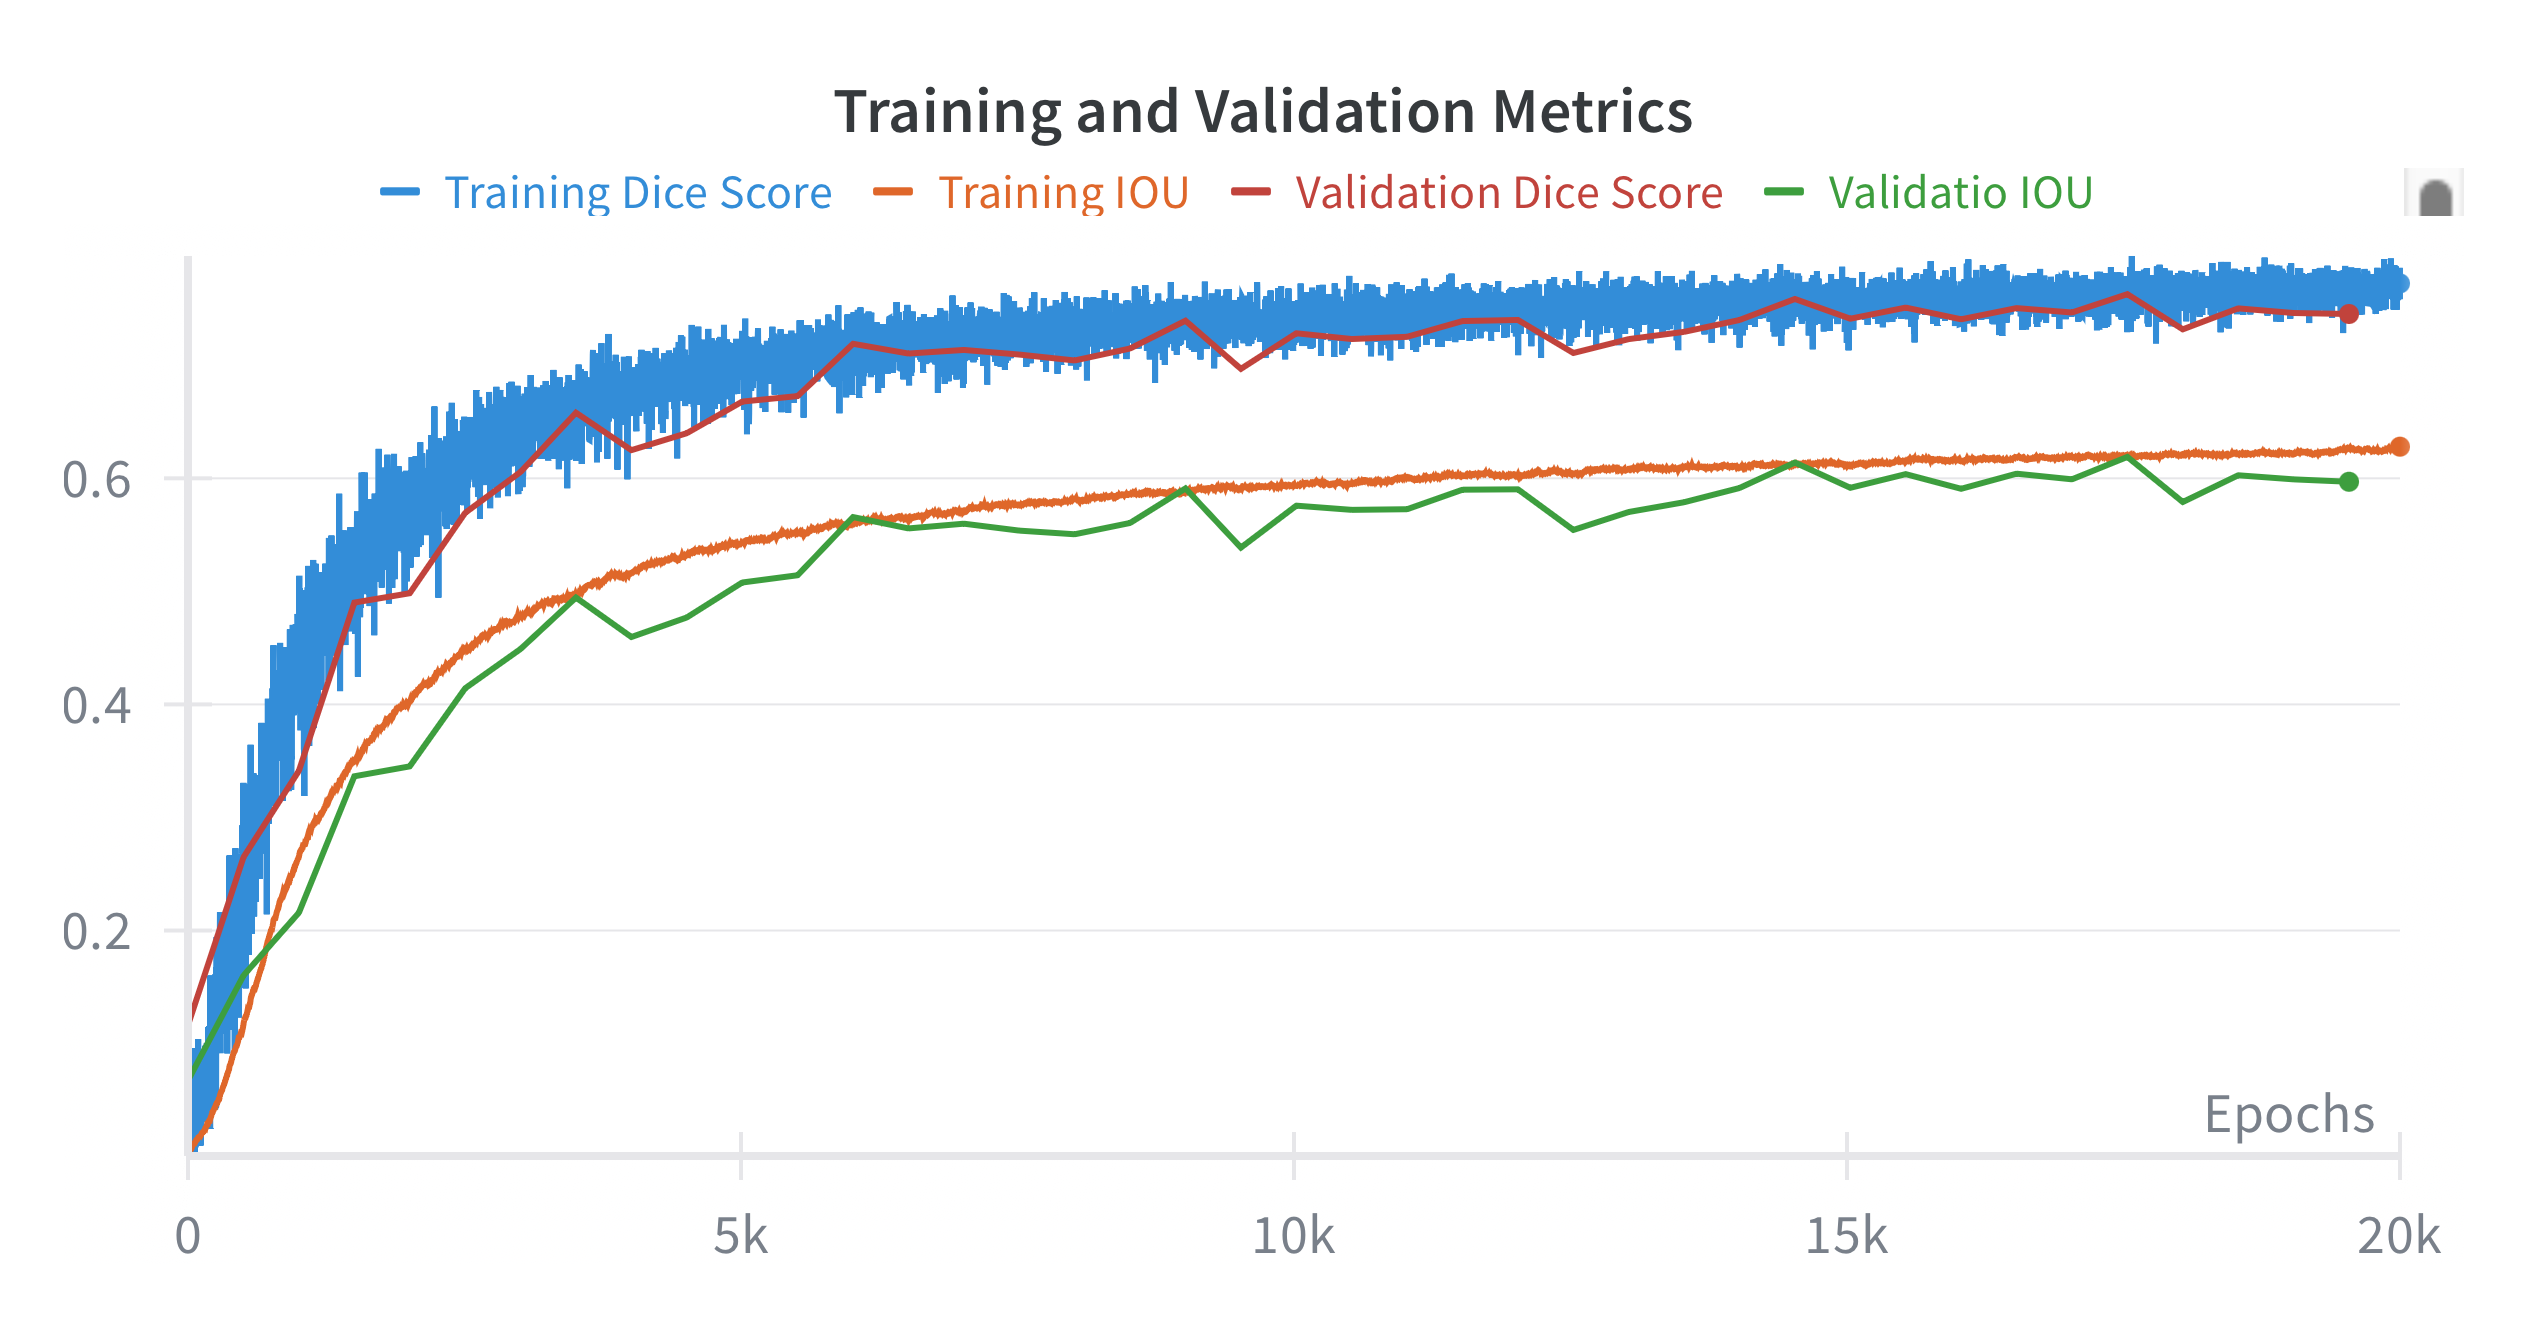
\includegraphics[width=0.8\textwidth]{figures/54_samv2_spines_metrics.png}
\captionof{figure}{Training and validation Dice score and IoU for SAMv2 spine fine-tuning.}
\label{fig:samv2_spine_training_validation}
\end{center}

The loss curves decrease steadily but remain noisier than in dendrite fine-tuning. Validation loss does not settle smoothly, suggesting that SAMv2 struggles with the higher variability and smaller scale of spines.

\begin{center}
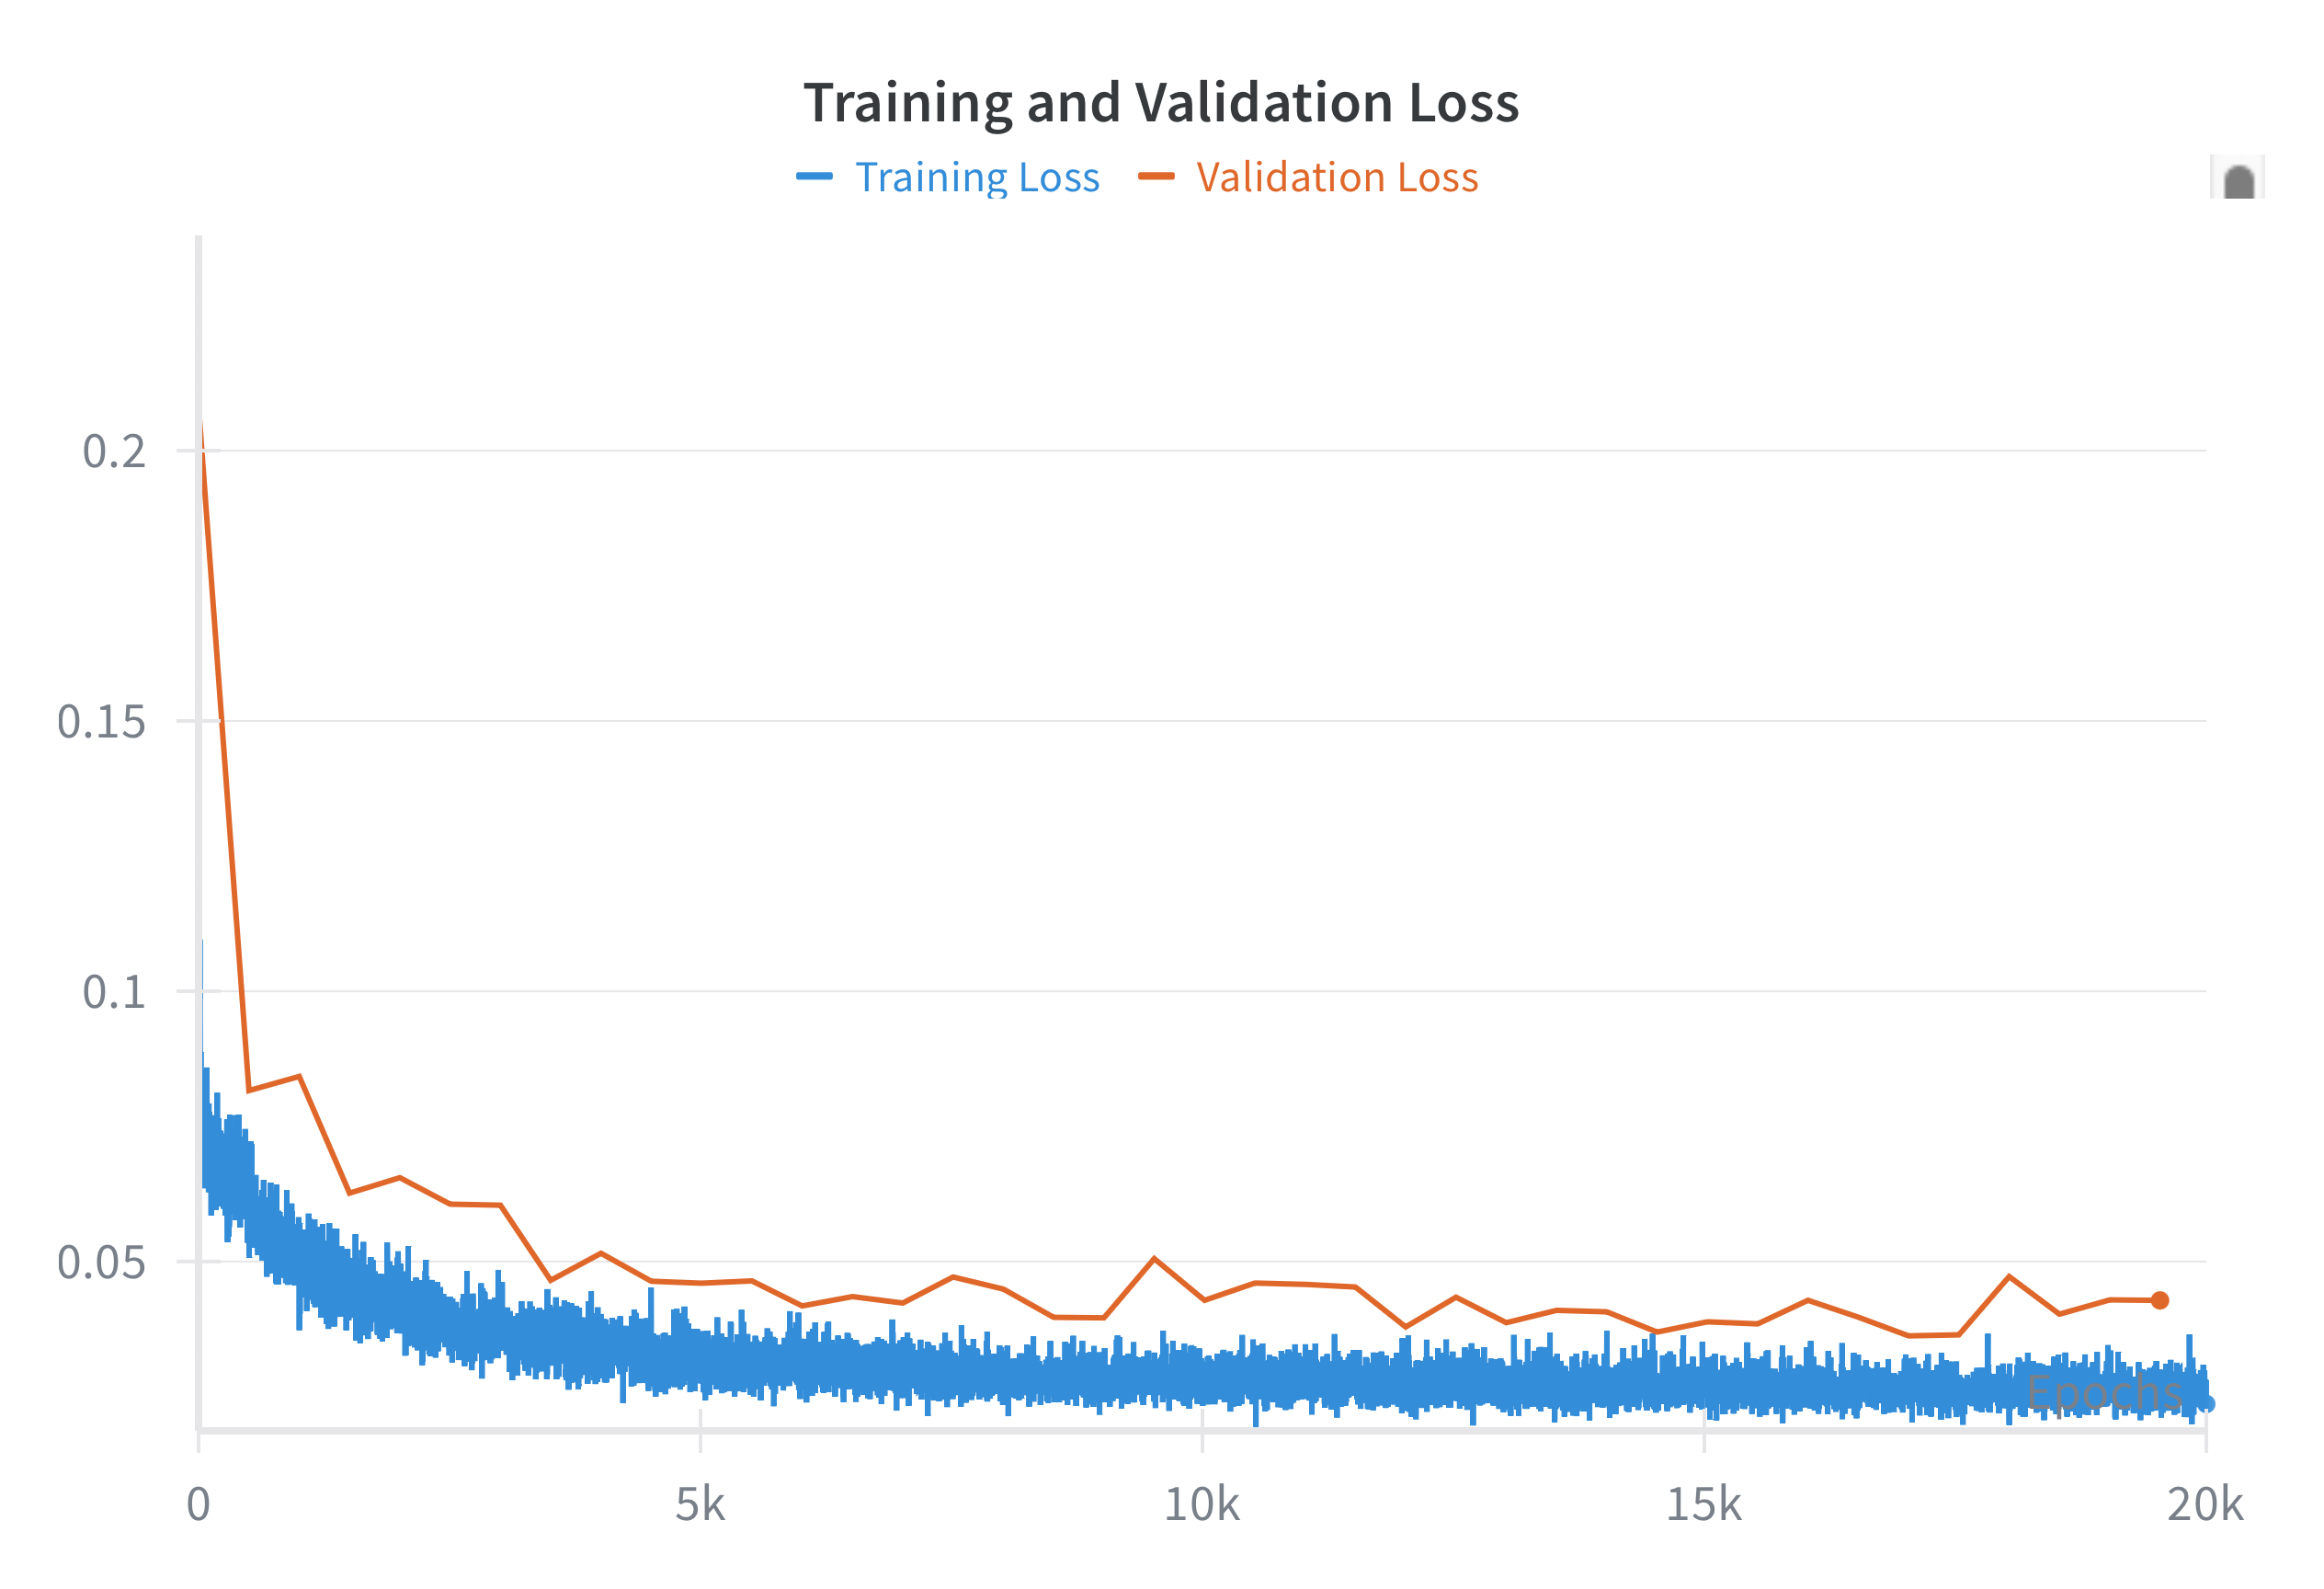
\includegraphics[width=0.8\textwidth]{figures/55_samv2_spines_loss.png}
\captionof{figure}{Training and validation loss for SAMv2 spine fine-tuning.}
\label{fig:samv2_dendrite_loss}
\end{center}